%!TEX root=../main.tex
\chapter{Clustering}\label{sec:clustering}

In clustering problems, we have a dataset of points in a multi-dimensional space, and we want to partition this dataset into a certain number of clusters, such that a certain distance or cost functions is minimized within the clusters and maximized among them.

In traditional approaches to this problem, the number of clusters $k$ is fixed in advance, and the algorithm partitions the dataset in the given number of clusters.\\
The best known algorithms of this type are:\label{clust-k-algs}
\begin{itemize}
    \item \textit{k-medians}: find the location of the $k$ centers as to minimize the average distance between a point and a center;
    \item \textit{k-centers}: find the location of the $k$ centers as to minimize the maximum distance between a point and a center;
    \item \textit{k-means}: find the location of the $k$ centers as to minimize the square of the distance between a point and a center;
\end{itemize}

\obs The most used is k-means, because its objective functions resembles variance, and so it can be interpreted as the search of Gaussians that randomly generated the points of the dataset.

\begin{thm}\label{thm:clustering-np}
    k-medians, k-centers and k-means are NP-complete problems.
\end{thm}

\begin{ex}
    We have a dataset of vectors representing users of a social network. Each vector could have up to millions dimensions (this is called \href{https://en.wikipedia.org/wiki/Curse_of_dimensionality}{\textit{curse of dimensionality}}), and we could have billions of such vectors.\\
    The distance between any pair of nodes tells us how much they are similar, so we want to cluster similar users to recommend them similar products or movies, or to send them similar ads.
\end{ex}

\begin{ex}
    We are Amazon and we have a dataset of users, each one with his/her geographic position in a map, so the distance between two points is the actual distance between two users. We have a fixed budget to position $k$ warehouses, and we want to find the best places where to put them.\\
    A good strategy could be to apply k-medians, so that each client, on average, is at the minimum possible distance from the warehouse.
\end{ex}

In real cases, often the number of clusters $k$ is not known \textit{a priori}, so one can use \textit{hierarchical clustering}, but this technique only produces some levels of grouping, so the user of the model still have to decide how many groups to use, and this is not always trivial.

\begin{ex}
    In the example in figure [\ref{fig:hierarchical-clustering-ex}] we can see that, after the algorithm groups the elements in levels of clusters, the user must decide which level to use, of if an intermediate number of clusters is preferable.
    
    \begin{figure}[h!]
        \centering
        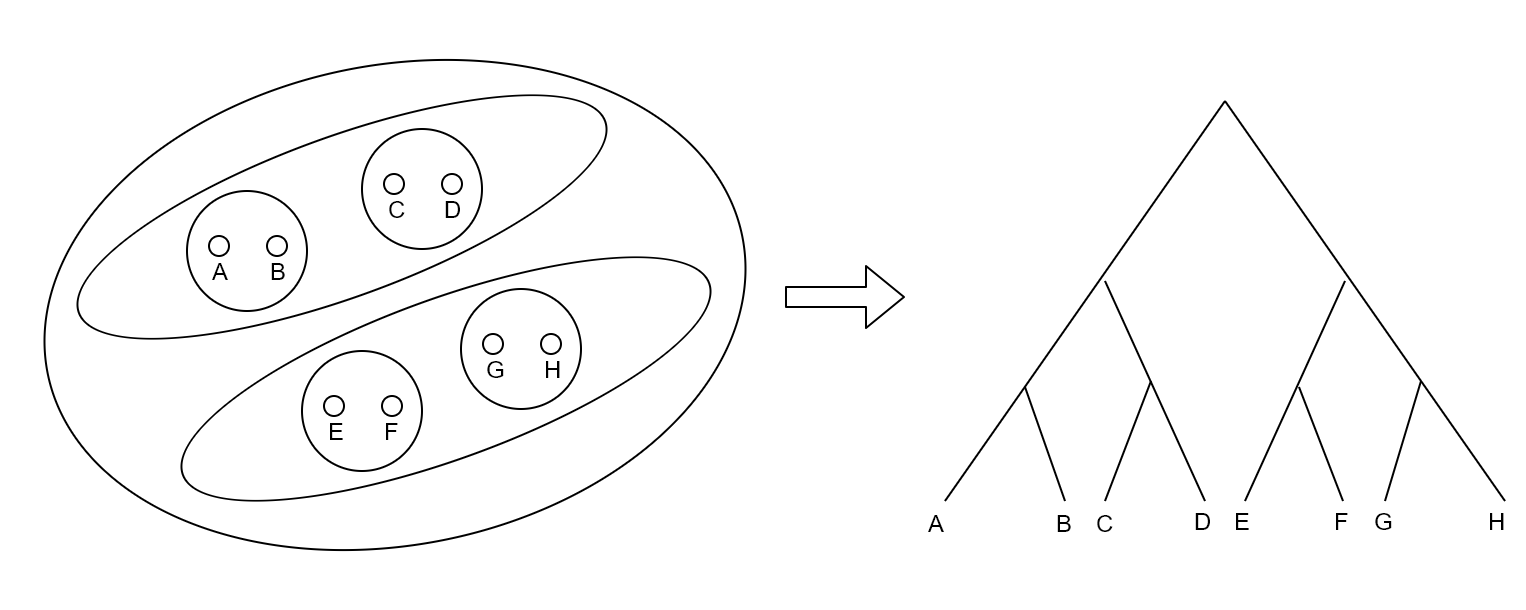
\includegraphics[width=0.7\textwidth]{hierarchical-clustering}
        \caption{An example of hierarchical clustering.}
        \label{fig:hierarchical-clustering-ex}
    \end{figure}
\end{ex}

As we will see, in \textit{correlation clustering} model it is the algorithm itself that produces the optimal number of clusters.\\ Generally speaking, if the user wants to minimize the distance within clusters, an optimal but useless solution would be to pick a singleton for each data point, whereas if the aim is to maximize the distance among clusters, one could end up with a single cluster that contains all the points, another optimal but useless solution, but these scenarios can't happen with correlation clustering.


\section{Correlation clustering}\label{sec:corr-clust}

We have a certain distance metric $d$ and a graph $G(V, E^+, E^-)$, where $E^+$ is the set of positive edges, that is, the ones that link nodes that are similar according to $d$, $E^-$ is the set of negative edges, that is, the ones that link dissimilar nodes according to $d$.\\
Note that $E^+ \cup E^- = \binom{V}{2}$ (i.e., the union of the edges in $E^+$ and $E^-$ is the set of all the edges connecting every pair of distinct vertices) and $E^+ \cap E^- = \emptyset$ (i.e., an edge can't be both positive and negative).\\
The goal is to put similar nodes together and different nodes separated, that is, we want to minimize the number of errors, given by the number of similar nodes put in different cluster and dissimilar nodes put in the same cluster, as formalized by the $cost$ function:

\begin{defn}[Cost]\label{def:clust-cost}
    Given a partition $\mathscr{C} = \{C_1, \ldots, C_i, \ldots\}$ of $V$ (that is, $C_i \cup C_j = \emptyset\ \forall\ i \neq j$, $\bigcup_{C_i \in \mathscr{C}} = V,\ C_i \neq \emptyset\ \forall\ C_i$), the $cost$ function is defined as follows:
    \begin{align}\label{eq:clust-cost}
        Cost(\mathscr{C}) = \sum_{\{i,j\} \in \binom{V}{2}} \bigl( &\left[ i,j \in E^+ \wedge\ i \text{ and } j \text{ are in different clusters of } \mathscr{C} \right] +\\
        &\left[ i,j \in E^- \wedge\ i \text{ and } j \text{ are in the same cluster of } \mathscr{C} \right] \bigr)\nonumber
    \end{align}
\end{defn}

\textbf{N.B.}: \textit{Even if there exist an edge connecting any pair of distinct vertices, in the following pictures sometimes we don't draw all the negative edges; so, if there isn't an edge between two nodes, we assume that there exists an implicit negative edge between those nodes.}

\begin{ex}
    Let's look at an example of correlation clustering in picture [\ref{fig:corr-clustering-ex}], where negative edges are dashed.
    
    \begin{figure}[h!]
        \centering
        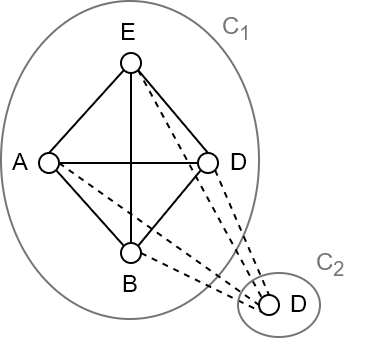
\includegraphics[width=0.3\textwidth]{corr-clustering}
        \caption{An example of correlation clustering.}
        \label{fig:corr-clustering-ex}
    \end{figure}

    In this case, we put the nodes $A, B, D, E$ together in cluster $C_1$ and we let node $C$ alone in cluster $C_2$, since the first nodes are all similar to each other, while the other is dissimilar from all the others.
\end{ex}

\begin{figure}[h!]
    \centering
    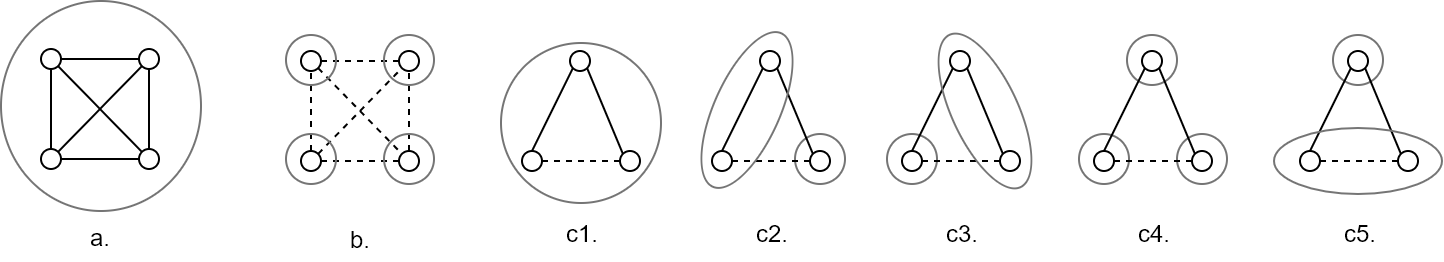
\includegraphics[width=\textwidth]{clust-special}
    \caption{Special cases in correlation clustering.}
    \label{fig:clust-special}
\end{figure}

Now we're interested in some \textbf{special cases}, shown in figure [\ref{fig:clust-special}]:
\renewcommand{\theenumi}{\alph{enumi}}
\begin{enumerate}
    \item If the nodes are all similar to each other, a single cluster will be created, and the \textit{cost} is 0;
    \item If nodes are all dissimilar to each other, a singleton for each node will be created, and the \textit{cost} is 0;
    \item If there are ``triangles'' like the ones in figures c1-c5, whatever clustering we produce the \textit{cost} is at least 1.
\end{enumerate}

These examples allow us to make some observations:
\begin{obs}\label{obs:clust-1}
    Since the solution can have $cost=0$, we can produce a multiplicative approximation only if we manage to always find the optimal solution if it has $cost=0$, otherwise the approximation will be infinite, even if the cost is small.
\end{obs}
\begin{obs}\label{obs:clust-2}
    We know that if the graph is composed of disjoint positive cliques, there exists a solution with $cost=0$, and we can find it by removing negative edges and looking for connected components. Thus, we can produce a multiplicative approximation.
\end{obs}
\begin{obs}\label{obs:clust-3}
    In whatever way we find triangles made of two positive edges and a negative edge, the $cost$ will be at least 1 for each such triangle, and for that reason those triangles are called ``\textit{bad triangles}'' (we will give a formal definition later).\\
    Furthermore, the $cost$ for each bad triangle is at least 1 even if there is a shared node between the bad triangles (see figure [\ref{fig:clust-bad-triangles}]a.), but it is 1/2 if there is a shared edge (see figure [\ref{fig:clust-bad-triangles}]b.).

    \begin{figure}[h!]
        \centering
        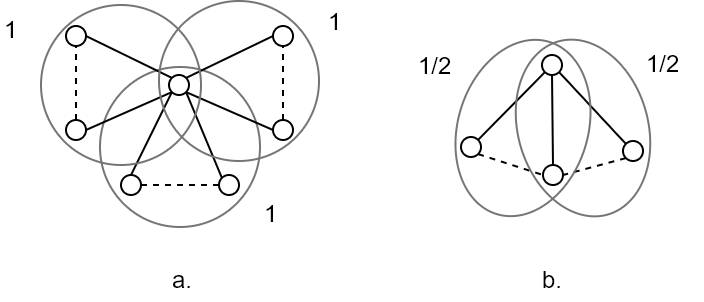
\includegraphics[width=\textwidth]{clust-bad-triangles}
        \caption{Cost of bad triangles.}
        \label{fig:clust-bad-triangles}
    \end{figure}

    Note that in figure [\ref{fig:clust-bad-triangles}] the gray circles represent bad triangles instead of clusters.
\end{obs}

\begin{defn}[Bad triangle]
    If $\{i,j\} \in E^+ \wedge \{j,k\} \in E^+ \wedge \{i,k\} \in E^-$, then $\{i,j,k\}$ is a bad triangle.
    
    The set of all the bad triangles of a graph is $\mathscr{T} = \left\{ \{i,j,k\} \st \{i,j,k\} \in \binom{V}{3} \text{ is a bad triangle} \right\}$.
\end{defn}


\subsection{Randomized pivot}\label{sec:random-pivot}

Now we present a greedy algorithm by Ailon, Charikar, Newman to approximate the correlation clustering problem:
\begin{lstlisting}[caption={Randomized Pivot}, label={lst:clust-random-pivot}]
randomized_pivot($V, E^+, E^-$):
    $V_1 \gets \emptyset$
    $i \gets 1$
    while $V_i \neq \emptyset$:
        pick $v_i \ \uar$ from $V_i$   // we choose the the pivot $v_i$
        $C_i \gets \left\{ w \st w \in V_i \wedge \{v_i, w\} \in E^+ \right\} \cup \{v_i\}$   // we create a new cluster $V_{i+1}$
        $V_{i+1} \gets V_i - C_i$   // we remove all the nodes of $V_{i+1}$
        $i \gets i+1$
    return $\mathscr{C}_G = \{C_1, C_2, \ldots, C_{i-1}\}$
\end{lstlisting}

\begin{ex}
    Let's look at some example of execution of Randomized Pivot.
    
    In figure [\ref{fig:clust-rp-1}] we can see all the steps performed by Randomized Pivot to obtain a good approximation of the correlation clustering problem: it produces three clusters, but with one error: there is a positive edge between clusters $C_2$ and $C_2$.
    \begin{figure}[h!]
        \centering
        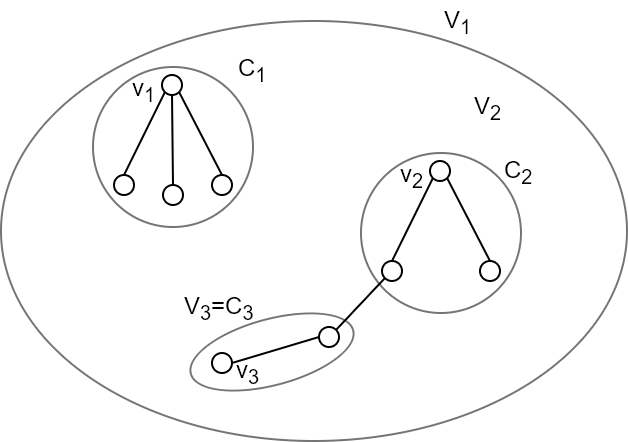
\includegraphics[width=0.5\textwidth]{clust-rp-1}
        \caption{Approximated solution of Randomized Pivot.}
        \label{fig:clust-rp-1}
    \end{figure}

    In figure [\ref{fig:clust-rp-2}] we can see that, if it exists, Randomized Pivot successes to obtain the optimal solution with $cost=0$: it creates a cluster for each clique, as previously said in observation [\ref{obs:clust-2}].
    \begin{figure}[h!]
        \centering
        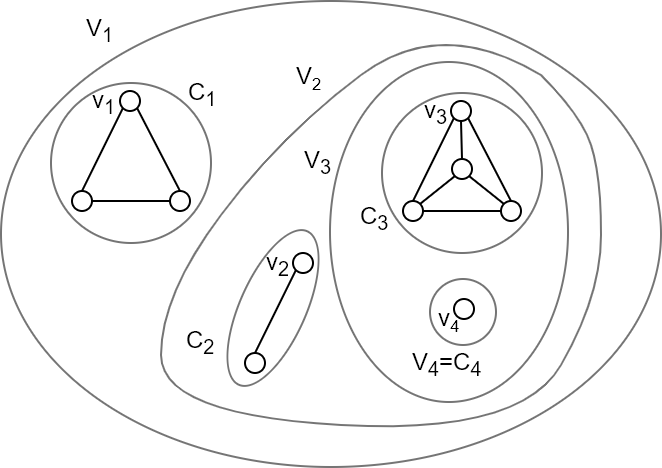
\includegraphics[width=0.5\textwidth]{clust-rp-2}
        \caption{Optimal solution of Randomized Pivot.}
        \label{fig:clust-rp-2}
    \end{figure}

    In figure [\ref{fig:clust-rp-3}] we see a case in which Randomized Pivot could find a very bad approximation: if there is a positive star, there are two possibilities:
    \renewcommand{\theenumi}{\alph{enumi}}
    \begin{enumerate}
        \item the algorithm chooses a leave of the star as pivot, so the $cost$ is only $n-1$;
        \item the algorithm chooses the root of the star as pivot, so the $cost$ is  even $\binom{n-1}{2} \approx n^2$.
    \end{enumerate}
    Note that the second (and worst) possibility happen with probability $1/n$, so it's not so unlikely.
    \begin{figure}[h!]
        \centering
        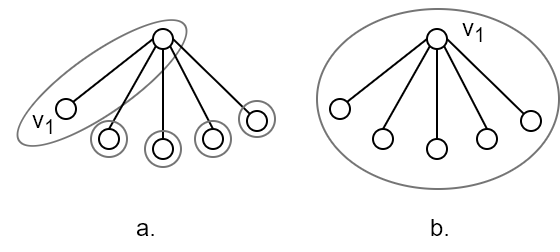
\includegraphics[width=0.5\textwidth]{clust-rp-3}
        \caption{Worst case of approximated solution of Randomized Pivot.}
        \label{fig:clust-rp-3}
    \end{figure}    
\end{ex}

\begin{thm}\label{thm:clust-rp-approx}
    Randomized Pivot [\ref{lst:clust-random-pivot}] returns an expected 3-approximation:
    \begin{equation}
        E\left[cost\left( \mathscr{C}_G \right)\right] \leq 3 \cdot \min_{\mathscr{C}} \{cost(\mathscr{C})\} = 3 \cdot OPT.
    \end{equation}
\end{thm}

\begin{obs}\label{obs:clust-4}
    By using Markov Inequality [\ref{eq:markov}], it can be proved that the bad event have small probability, if we execute the algorithm many times:
    \begin{itemize}
        \item Let $X=cost(\mathscr{C})$, $X$ is a not concentrated random variable with expected value $E[X] \leq 3 \cdot OPT$;
        \item $\Pr{X \geq 3 \cdot c \cdot OPT} \leq \Pr{X \geq c \cdot E[X]} \leq \frac{1}{c}$;
        \item If we pick $c=1+\frac{\varepsilon}{3}$, then $\Pr{X \geq (3 + \varepsilon) \cdot OPT} \leq \frac{1}{1 + \varepsilon / 3} = 1 - \Theta(\varepsilon)$;
        \item Thus, if we execute the algorithm $\frac{1}{\Theta(\varepsilon)}$ times, the probability of the bad event becomes small:\\
        $\left( 1 - \Theta(\varepsilon) \right)^{\left( \frac{\ln 1/\delta}{\varepsilon} \right)} \to \Theta(\delta)$;
        \item At this point, it is sufficient to return the best solution among those computed by the algorithm in the various trials, and with high probability it will be a solution that respects the 3-approximation, that is, a solution for which the bad event doesn't happen.
    \end{itemize}
\end{obs}

\begin{proof}[Proof of Theorem \ref{thm:clust-rp-approx}]
    As usual, we will prove the theorem by steps, introducing some lemmas and claims.
    
    \begin{lem}\label{l:clust-1}
        Let $cost^+_j := \abs{\big\{ \{v,w\} \st v \in C_j \wedge w \in V_{j+1} \wedge \{v,w\} \in E^+ \big\}}$ and\\ $cost^-_j := \abs{\big\{ \{v,w\} \st v,w \in C_j \wedge \{v,w\} \in E^- \big\}}$, then
        \begin{equation}
            cost(\mathscr{C}_G) = \sum_j \left( cost_j^+ + cost_j^- \right).
        \end{equation}
    \end{lem}
    \begin{proof}
        The proof directly follows from the definition of $cost_j^+$ and $cost_j^-$: as we can see in figure [\ref{fig:clust-costs}], $cost_j^+$ covers the first part of the definition of $cost$ [\ref{eq:clust-cost}], that is, the cases in which the algorithm puts two similar nodes in different clusters (edges marked with $*$ in the picture), and $cost_j^-$ covers the second part of the definition, i.e., the cases in which two dissimilar nodes are put in the same cluster (edges marked with $**$ in the picture). Thus, all the errors (red edges) are covered either by $cost_j^+$ or by $cost_j^-$.
    \end{proof}

    \begin{figure}[h!]
        \centering
        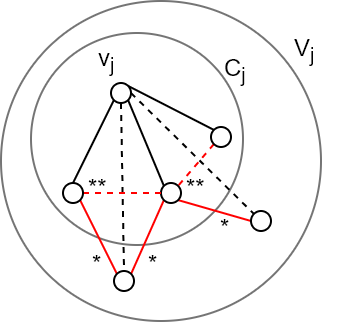
\includegraphics[width=0.35\textwidth]{clust-costs}
        \caption{Example of application of the definition of $cost_j^+$ and $cost_j^-$.}
        \label{fig:clust-costs}
    \end{figure}

    The following two claims, that follow from Lemma [\ref{l:clust-1}], connect the different types of bad triangles we see in figure [\ref{fig:clust-costs}] with the different types of errors, or costs.
    
    \begin{claim}\label{cl:clust-1}
        $cost_j^+$ is the number of bad triangles $T$ that
        \begin{enumerate}
            \item are fully contained in $V_j$,
            \item contain $v_j$, and
            \item for which $\abs{C_j \cup T} = 2$.
        \end{enumerate}
    \end{claim}

    \begin{claim}\label{cl:clust-2}
        $cost_j^-$ is the number of bad triangles $T$ that
        \begin{enumerate}
            \item are fully contained in $C_j \subseteq V_j$,
            \item contain $v_j$.
        \end{enumerate}
    \end{claim}

    Now we introduce the concept of ``hitting'' a bad triangle, that will be useful to prove the next lemma.
    \begin{defn}[Hit]\label{def:clust-hit}
        We say that Random-Pivot [\ref{lst:clust-random-pivot}] \emph{hits} a bad triangle $T$ if $\exists\ j \st T \subseteq V_j$ and $v_j \in T$.
    \end{defn}

    \begin{cor}\label{cor:clust-1}
        $cost(\mathscr{C}_G)$ is the number of bad triangles hit by Random-Pivot.
    \end{cor}
    \begin{proof}
        Corollary [\ref{cor:clust-1}] follows by the claims [\ref{cl:clust-1}] and [\ref{cl:clust-2}] and by the definition of ``hit'' [\ref{def:clust-hit}].
    \end{proof}
    
    We introduced the concept of \textit{hitting} because we want to relate the probability of hitting a bad triangle with the cost paid by the algorithm. We can't directly compute this probability, but we obtain a useful linear relationship.
    \begin{lem}\label{l:clust-2}
        Given a bad triangle $T \in \mathscr{T}$, let $p_T$ be the (a priori) probability that Random-Pivot will hit $T$. Then
        \begin{equation}
            E[cost(\mathscr{C}_G)] = \sum_{T \in \mathscr{T}} p_T.
        \end{equation}
    \end{lem}
    \begin{proof}
        Lemma [\ref{l:clust-2}] follows by Corollary [\ref{cor:clust-1}] and the definition of expected value [\ref{def:expected-value}]: we know that $cost(\mathscr{C}_G)$ is a random variable (it depends on $\mathscr{C}_G$, that is the result returned by Randomized Pivot, that in turn is a random algorithm, as the name suggests), and, since its value is the number of bad triangles hit by the algorithm, we can decompose it in a sum of Bernoulli random variables $X_T$, one for each $T \in \mathscr{T}$, that assume value 1 if the algorithm hits $T$, with probability $p_T$, and 0 otherwise.
    \end{proof}

    So, finally we have all the tools we need to prove that $E\left[cost\left( \mathscr{C}_G \right)\right] \leq 3 \cdot OPT$ (the claim of Theorem [\ref{thm:clust-rp-approx}]), that is, $\frac{\sum_{T \in \mathscr{T}} p_T}{3} \leq OPT$, and we'll do it with a primal-dual proof, exploiting the linear program underlying Randomized-Pivot.
    
    We begin with the dual LP:
    \begin{equation}\label{lp:clust-dual}
        \begin{aligned}
            &\min \sum_{\{i,j\} \in \binom{V}{2}} X_{\{i,j\}}&\\
            &\begin{cases}
                X_{\{i,j\}} + X_{\{j,k\}} + X_{\{i,k\}} \geq 1 & \forall\ \{i,j,k\} \in \mathscr{T}
            \end{cases}&\\
            &X_{\{i,j\}} \geq 0 \ \forall\ \{i,j\} \in \binom{V}{2}&
        \end{aligned}
    \end{equation}
    
    \obs The objective function is the number of errors the algorithm makes (that is, the cost function), while the meaning of the constraint is that the sum of the costs paid for a bad triangle is at least 1, since we know we will make at least one error for each bad triangle.
    
    \begin{lem}\label{l:clust-3}
        For each solution $\mathscr{C}$, $cost(\mathscr{C}) \geq \text{DUAL}^*$, where $\text{DUAL}^*$ is the optimal solution of the dual LP.
    \end{lem}
    \begin{proof}
        It is hard to find the optimal solution of the dual, but for our purpose it is sufficient to show a feasible solution and it will be greater or equal than the optimal one.
        
        Let $X_{\{i,j\}} := \begin{cases}
        1 & \text{if } \big( \{i,j\} \in E^+ \wedge i \text{ and } j \text{ are split by } \mathscr{C} \big) \text{ or }\\
        &\phantom{\text{if }} \big( \{i,j\} \in E^- \wedge i \text{ and } j \text{ are together in } \mathscr{C} \big)\\
        0 & \text{otherwise}
        \end{cases}$.\\
        Informally, $X_{\{i,j\}}=1$ iff there is an error in $\mathscr{C}$.
        
        This is a feasible solution because we are counting each bad triangle, and so the value of the dual, with this solution, is equal to $cost(\mathscr{C})$.
    \end{proof}
    
    \begin{cor}\label{cor:clust-2}
        \begin{equation}
            OPT \geq \text{DUAL}^*
        \end{equation}
    \end{cor}
    \begin{proof}
        Since $OPT = \min_{\mathscr{C}} \{cost(\mathscr{C})\}$, the corollary follows directly from Lemma [\ref{l:clust-3}].
    \end{proof}

    Now we are going to present the primal LP and to show that $\frac{p_T}{3}$ is a feasible solution. This will allow us to conclude that the following inequality holds:
    \begin{claim}\label{cl:clust-ineq}
        \begin{equation}\label{eq:clust-ineq}
            \frac13 \cdot \text{E}[\text{cost}(\mathscr{C}_P)] =  \sum_{T \in \mathscr{T}} \frac{p_T}{3} \leq \text{PRIMAL}^* \leq \text{DUAL}^* \leq OPT
        \end{equation}
    \end{claim}

    \obs\label{obs:clust-ineq} If we prove the first inequality, we will have proved that the expected cost of the solution returned by the algorithm is no more than 3 times the cost of the optimal solution. Note that this concludes the proof of Theorem [\ref{thm:clust-rp-approx}].
    
    \begin{proof}
        The first equation follows from Lemma~\ref{l:clust-2}, the second inequality is due to the weak duality theorem [\ref{thm:weak-duality}], the third one to Corollary [\ref{cor:clust-2}], and we'll prove the first one shortly with Lemma [\ref{l:clust-4}].
    
        Primal LP:
        \begin{equation}\label{lp:clust-primal}
            \begin{aligned}
                &\max \sum_{T \in \mathscr{T}} y_T&\\
                &\begin{cases}
                    \sum_{T \in \mathscr{T},\ \{i,j\} \subset T} y_T \leq 1 & \forall\ \{i,j\} \in \binom{V}{2}
                \end{cases}&\\
                &y_T \geq 0 \ \forall\ T \in \mathscr{T}&
            \end{aligned}
        \end{equation}
        
        \obs This kind of constraint is called \textit{fractional packing of triangles}: for each edge, we want to take at most a weight of 1, summing up the weights of the bad triangles that contain that edge.
    
        Consider the primal program, and set $y_T = p_T / 3$ for each $T \in \mathscr{T}$. This solution has a value of $\frac13 \cdot \sum_{T \in \mathscr{T}} p_T$ in the primal so, if we prove it is feasible for the primal, we have shown that $\frac13 \cdot \sum_{T \in \mathscr{T}} p_T \le \pi^{*}$, where $\pi^{*}$ is the solution of the primal.
    
        \begin{lem}\label{l:clust-4}
            $y_T = \frac{p_T}{3}$ is a feasible solution for the primal.
        \end{lem}
    
        \begin{proof}
            To conclude that the solution is feasible for the primal, we only have to prove that, for each $\{i,j\} \in \binom V2$, it holds
            $\sum_{\substack{T \in \mathscr{T}\\T \supset \{i,j\}}} y_T \le 1$.
        
            Fix an edge $\{i,j\} \in \binom V2$, and let $A = \bigcup_{\substack{T \in \mathscr{T}\\T \supset \{i,j\}}} T$ be the set of each node of each bad triangle that includes the edge $\{i,j\}$. Let $\xi$ be the event that, during a run of the algorithm, at least one node of $A$ becomes a pivot.\\
            Note that we need $\xi$ because we know that, if it happens, the algorithm will find at least a triangle in $A$, otherwise none, and this allows us to divide the probabilities in two parts, by lat of total probability.
        
            Then,
            \begin{flalign*}
                \sum_{\substack{T \in \mathscr{T}\\T \supset \{i,j\}}} y_T &= \sum_{\substack{T \in \mathscr{T}\\T \supset \{i,j\}}} \frac{p_T}3&\\
                &=\frac13 \cdot \sum_{\substack{T \in \mathscr{T}\\T \supset \{i,j\}}} \Pr{T \text{ is hit}}&\\
                &=\frac13 \cdot \sum_{\substack{T \in \mathscr{T}\\T \supset \{i,j\}}} \Big( \Pr{T \text{ is hit} \mid \xi} \cdot \Pr{\xi} +  \Pr{T \text{ is hit} \mid \overline{\xi}\,} \cdot \Pr{\,\overline{\xi}\,} \Big)&\tag{by total probability}\\
                &=\frac13 \cdot \sum_{\substack{T \in \mathscr{T}\\T \supset \{i,j\}}} \Big( \Pr{T \text{ is hit} \mid \xi} \cdot \Pr{\xi} + 0 \cdot \Pr{\,\overline{\xi}\,}\Big)&\\
                &=\frac13 \cdot \sum_{\substack{T \in \mathscr{T}\\T \supset \{i,j\}}} \Big( \Pr{T \text{ is hit} \mid \xi} \cdot \Pr{\xi}\Big)&\\
                &\le \frac13 \cdot \sum_{\substack{T \in \mathscr{T}\\T \supset \{i,j\}}} \Pr{T \text{ is hit} \mid \xi}.&
            \end{flalign*}
            Under the conditioning $\xi$, there will be one node that ends up being the first  pivot chosen in $A$; suppose it is $v_k$ (that is, let $k$ be such that $v_k \in A$ and $v_{k'} \not\in A$ fo each $1 \le k' < k$ --- observe that such a $k$ must exists if $\xi$ happens).
            Moreover, let $B = V_k \cap A$ be the subset of nodes of $A$ that are part of the residual graph when $v_k$ is chosen as a pivot.
        
            Then,
            \begin{flalign*}
                \sum_{\substack{T \in \mathscr{T}\\T \supset \{i,j\}}} y_T &\le \frac13 \cdot \sum_{\substack{T \in \mathscr{T}\\T \supset \{i,j\}}} \Pr{T \text{ is hit} \mid \xi}&\\
                &=\frac13 \cdot \sum_{S \subseteq A} \left(\Pr{B = S \mid \xi} \cdot \sum_{\substack{T \in \mathscr{T}\\T \supset \{i,j\}}} \Pr{T \text{ is hit} \mid B = S \wedge \xi}\right)&\tag{$*^1$}\\
                &=\frac13 \cdot \sum_{S \subseteq A} \left(\Pr{B = S \mid \xi} \cdot \left(\sum_{\substack{T \in \mathscr{T}\\ \{i,j\} \subset T  \subseteq S}} \Pr{T \text{ is hit} \mid B = S \wedge \xi} + \sum_{\substack{T \in \mathscr{T}\\ \{i,j\} \subset T  \not\subseteq S}} \Pr{T \text{ is hit} \mid B = S \wedge \xi}\right)\right)&\tag{$*^2$}\\
                &=\frac13 \cdot \sum_{S \subseteq A} \left(\Pr{B = S \mid \xi} \cdot \left(\sum_{\substack{T \in \mathscr{T}\\ \{i,j\} \subset T  \subseteq S}} \Pr{T \text{ is hit} \mid B = S \wedge \xi} + \sum_{\substack{T \in \mathscr{T}\\ \{i,j\} \subset T  \not\subseteq S}} 0\right)\right)\tag{$*^3$}&\\
                &=\frac13 \cdot \sum_{S \subseteq A} \left(\Pr{B = S \mid \xi} \cdot \sum_{\substack{T \in \mathscr{T}\\ \{i,j\} \subset T  \subseteq S}} \Pr{T \text{ is hit} \mid B = S \wedge \xi} \right)&\\
                &=\frac13 \cdot \sum_{S \subseteq A} \left(\Pr{B = S \mid \xi} \cdot \sum_{\substack{T \in \mathscr{T}\\ \{i,j\} \subset T  \subseteq S}}  \frac3{|S|} \right)\tag{$*^4$}&\\
                &=\frac13 \cdot \sum_{S \subseteq A} \left(\Pr{B = S \mid \xi} \cdot (|S| -2) \cdot  \frac3{|S|} \right)&\\
                &\le\frac13 \cdot \sum_{S \subseteq A} \Big(\Pr{B = S \mid \xi} \cdot 3 \Big)&\tag{we upper bound $\frac{|S|-2}{|S|}$ with 1}\\
                &=\sum_{S \subseteq A} \left(\Pr{B = S \mid \xi} \right) = \Pr{B \subseteq A\mid \xi}= 1.&
            \end{flalign*}
            
            In $(*^1)$ we apply the law of total probability again, to split the probabilities according to the value of $B$; in $(*^2)$ we break the sum in two parts, with triangles completely in $S$ and \textit{not} completely in $S$, the latter will never be hit by the algorithm, by definition of hit [\ref{def:clust-hit}], (so their probabilities are 0 in $(*^3)$), the former have probability $3/|S|$ of being hit, since each of their vertexes has the same probability of being chosen as the pivot (since it's picked $\uar$), and we use it in $(*^4)$.
            
            Thus, the generic constraint of the primal is satisfied: the proposed primal solution is then feasible, which concludes the proof of Lemma [\ref{l:clust-4}].
        \end{proof}
        
        Then, $\frac13 \cdot \sum_{T \in \mathscr{T}} p_T$ cannot be larger than the optimal primal value $\pi^*$. The proof of Claim [\ref{cl:clust-ineq}] is concluded.
    \end{proof}
    
    By Claim [\ref{cl:clust-ineq}], we have
    $E[\text{cost}(\mathscr{C}_P)] \le 3 \cdot \text{cost}(\mathscr{C}^{\star})$, that concludes the proof of Theorem [\ref{thm:clust-rp-approx}], as observed in [\ref{obs:clust-ineq}].
\end{proof}    


\subsection{Parallel Random Pivot}

\obs The random-pivot algorithm [\ref{lst:clust-random-pivot}] can be very slow if there are many isolated nodes (i.e., many negative edges).

The good news is we can obtain a $(3+\varepsilon)-approximation$ in logarithmic time, if we run a parallel version of the algorithm in a framework such as Pregel or Map-Reduce.\\
The algorithm is deeply discussed and analyzed in the paper \href{https://dl.acm.org/citation.cfm?id=2623743}{Correlation clustering in MapReduce}, by Chierichetti et al., here we just purpose a brief description.

\begin{lstlisting}[caption={Parallel Randomized Pivot}, label={lst:parallel-random-pivot}]
parallel randomized pivot:
    while istance is not empty:
        - $\Delta^+ \gets$ max positive degree;
        - activate each element with probability $\varepsilon/\Delta^+$;
        - deactivate active nodes liked to other active nodes;
        - create a cluster for each remaining active node   // there are many pivots
          (break ties randomly);
\end{lstlisting}

\begin{thm}
    $\Delta^+$ is halved after $1/3 \cdot \log(n)$ iterations.
\end{thm}

\obs The probability $\frac{\varepsilon}{\Delta^+}$ is higher for nodes with higher degree, but those nodes have more neighbors that could deactivate them, so there is a balancing between these two aspects.

Open problem: How to handle the case where there are neither positive nor negative edges? I.e., in which, for some pairs of nodes, we don't know if the two elements are similar or dissimilar.


\section{K-Centers}\label{sec:k-centers}

As we briefly saw at the beginning of this chapter [\ref{clust-k-algs}], the goal of k-centers problem is to find the location of the $k$ centers as to minimize the maximum distance between a point and a center. Now we'll define the problem more formally and we'll give an algorithm to approximate its solution.

\begin{defn}[Minimum k-centers]\label{defn:k-centers}
    The minimum k-centers problem is defined as follows:\\
    Input: $X = \{x_1, x_2, ..., x_n\}$ points in a metric space.\\
    Goal: Find $C \subseteq X$ such that $|C| = k$ and $\max_{x \in X} d(x,C)$ is minimized, where $d(x,C) := \min_{y \in C} d(x,y)$ is the distance between a point and a set of points.\\
    Using the value of $d(x,C)$, we can rewrite the goal as: Minimize $\max_{x \in X} \min_{y \in C} d(x, y)$.
\end{defn}

As we stated in the introduction [\ref{thm:clustering-np}], minimum k-centers is np-complete, so we look for an approximation. It has been proved that the best possible approximation one can obtain in polynomial time is a 2-approximation: $$OPT \leq A(X,k) \leq 2 OPT \ \ \ \forall\ X,k.$$

Now we present the algorithm to solve the minimum k-centers problem, then we'll prove it gives a 2-approximation.

\begin{lstlisting}[caption={Minimum k-centers}, label={lst:min-k-centers}]
min-k-centers:
    $C \gets \{ \text{any point} \}$
    for $i = 2, \ldots, k$:
        let $x$ be such that $d(x,C)$ is maximized
        $C \gets C \cup \{x\}$
    return $C$
\end{lstlisting}

\begin{thm}\label{thm:k-centers-approx}
    Min-k-centers algorithm [\ref{lst:min-k-centers}] returns a 2-approximation for the minimum k-centers clustering problem.\\
    In other words, $\forall\ x \in X,\ d(x,C) \leq 2 \cdot OPT$.
\end{thm}
\begin{proof}
    Let $C = \{c_1, c_2, \ldots, c_k\}$ be the set of centers chosen by the algorithm, where the indexes follows the order in which they are chosen.
    
    Assume, by contradiction, that $C$ is not a 2-approximation, then 
    \begin{equation}\label{eq:centers-assumption}
        \exists\ z \text{ s.t. } d(z, C) > 2 \cdot OPT.
    \end{equation}
    
    If we prove that the following claim holds under this assumption, we will reach an absurd, so we'll prove the theorem.
    \begin{claim}\label{cl:centers}
        $d(c_i, c_j) > 2 \cdot OPT\ \forall\ i,j$.
    \end{claim}
    \begin{proof}[Proof of claim \ref{cl:centers}]
        \begin{obs}
            $\forall\ A \subset C,\ d(z,A) \geq d(z,C)$, since we have more possibilities to find a point closer to $z$ in $C$ than in $A$ (since it's bigger).
        \end{obs}
        We can use this observation and our assumption [\ref{eq:centers-assumption}] to show that $d(z, \{c_1\}) \geq d(z,C) > 2 \cdot OPT$.\\
        Since the algorithm [\ref{lst:min-k-centers}] pick as center the furthest point from those already considered, we also know that $d(c_2, \{c_1\}) \geq d(z, \{c_1\})$.
        
        Similarly, we can say that $d(c_3, \{c_1, c_2\}) \geq d(z, \{c_1, c_2\}) \geq d(z,C) > 2 \cdot OPT$.
        The same holds for $c_4$: $d(c_4, \{c_1, c_2, c_3\}) \geq d(z, \{c_1, c_2, c_3\}) > 2 \cdot OPT$.
        And so on for each $c_i$ up to $c_k$.
    \end{proof}

    Now we can go back to the proof of Theorem [\ref{thm:k-centers-approx}], and show that the claim [\ref{cl:centers}], true under assumption [\ref{eq:centers-assumption}], produces a contradiction.
    
    Let $O = \{o_1, o_2, \ldots, o_k\}$. Any point in the dataset must be at distance at most $OPT$ from a center in $O$, by definition of the problem; the same holds for the points in $C$, so let's pick $c_1$ from $C$ and let's say that the closest point to $c_1$ in $O$ is $o_1$ (it's just a name). Then $c_2$ can't be at distance $\leq OPT$ from $o_1$, otherwise we have $d(c_1, c_2) \leq 2 \cdot OPT$, but it's impossible for [\ref{cl:centers}].
    
    The same holds for any $c_i \in C$, thus each $c_i$ is ``covered'' by a different $o_i$.
    
    Then, $z$ can't be covered by any $o_i$, which is a contradiction.
\end{proof}
